\section{Realizing the Proposed Error Confinement in a RISC Processor} \label{sec:qos_asip}
The proposed Error-Confinement function requires a scheme for detecting a memory error 
for providing the needed a-priori information $\setF$ and a look up table for storing the 
expected reference values to be used for replacing the erroneous data. Obviously the realization of such a scheme 
in a processor require i) the introduction of custom instructions and ii) micro-architectural enhancements that we discuss next.     

We base the proposed enhancements on the RISC processor core IP from Synopsys Processor Designer, 
which consists of five pipeline stages as depicted in Figure \ref{fig:qos_processor},  
supports mixed 16/32 bits instructions, while the HDL implementation of the core is fully synthesizable. 
Note that for the detection of an error required in our scheme we propose the use of a single parity bit within each word which is sufficient for detecting a single error. By doing so we essentially limit the required overhead as opposed to ECC methods  that require the addition of several parity bits for the detection and correction of a single or more errors.     

\subsection{Custom Instructions}
At the assembly level we introduce 4 new instructions, which can be used either in standalone assembly or be embedded as inline assembly in a high-level language such as C/C++.
%\begin{enumerate}
% \item 
 To begin with we need to specify  the start address and the word size of the memory block that is going to be protected by the proposed scheme and indicate the place in the look up table (LUT) as well its size, where the expected value to be used in case of an error is stored. To this end we introduce the following instruction:     
  \textit{\textbf{set\_data @\{data\_start\} @\{data\_size\} @\{lut\_start\} @\{lut\_size\}}} \\
in which all arguments are provided using general purpose registers.
% \item 

Furthermore, the instruction \textit{\textbf{chk\_load @\{dst\} @\{src\} @\{index\}}} is introduced for 
statistically confining the error in specific memory blocks while performing memory reads . In particular, before reading the protected data, this instruction detects any error within the read data in the register @\{src\} and in case i) of an error it replaces the erroneous data with the reference expected value stored in the position @\{index\} of the LUT and loads the value
into the register @\{dst\}, while ii) in case of no error the register @\{dst\} is assigned directly to the correct value kept in the register @\{src\}.

Finally, to enable the protection of specific memory write accesses we introduce 
the instruction \textit{\textbf{en\_parity}} as well as the instruction  \textit{\textbf{dis\_parity}} 
for disabling the protection of any data if needed. The above instructions are incorporated in the newly constructed LLVM based C compiler (through the use of Synopsys Processor Designer), which supports instruction set extensions using inline assembly.

%\end{enumerate}

%\subsection{Programming Example}
%We show the corresponding programming model with the DCT application as an example, which is briefly listed in Figure %\ref{fig:qos_program}. The example declares an 2D array containing 64 reference DCT coefficients and register it as the protection array for the image of size $512 \times 512$. In the DCT function, before a value is written to the DCT memory, the protection is turned on to enable parity encoding, which is again turned off after write access. In the quantization function, the load check is performed whenever a value is read out from the array of DCT coefficients for possible correction. Further algorithms which exhibit the feature of data approximation can directly follow the example in Figure \ref{fig:qos_program}.

\subsection{Micro-Architectural Enhancements}

The introduced instructions require the enhancement of the microarchitecture of the target RISC processor with customized modules   
which are highlighted in Figure \ref{fig:qos_processor}. The detailed functionality of the logic functions within each module in each pipeline stage is described in detail in Figure \ref{fig:qos_arch_explain}.

\begin{figure}
\centering
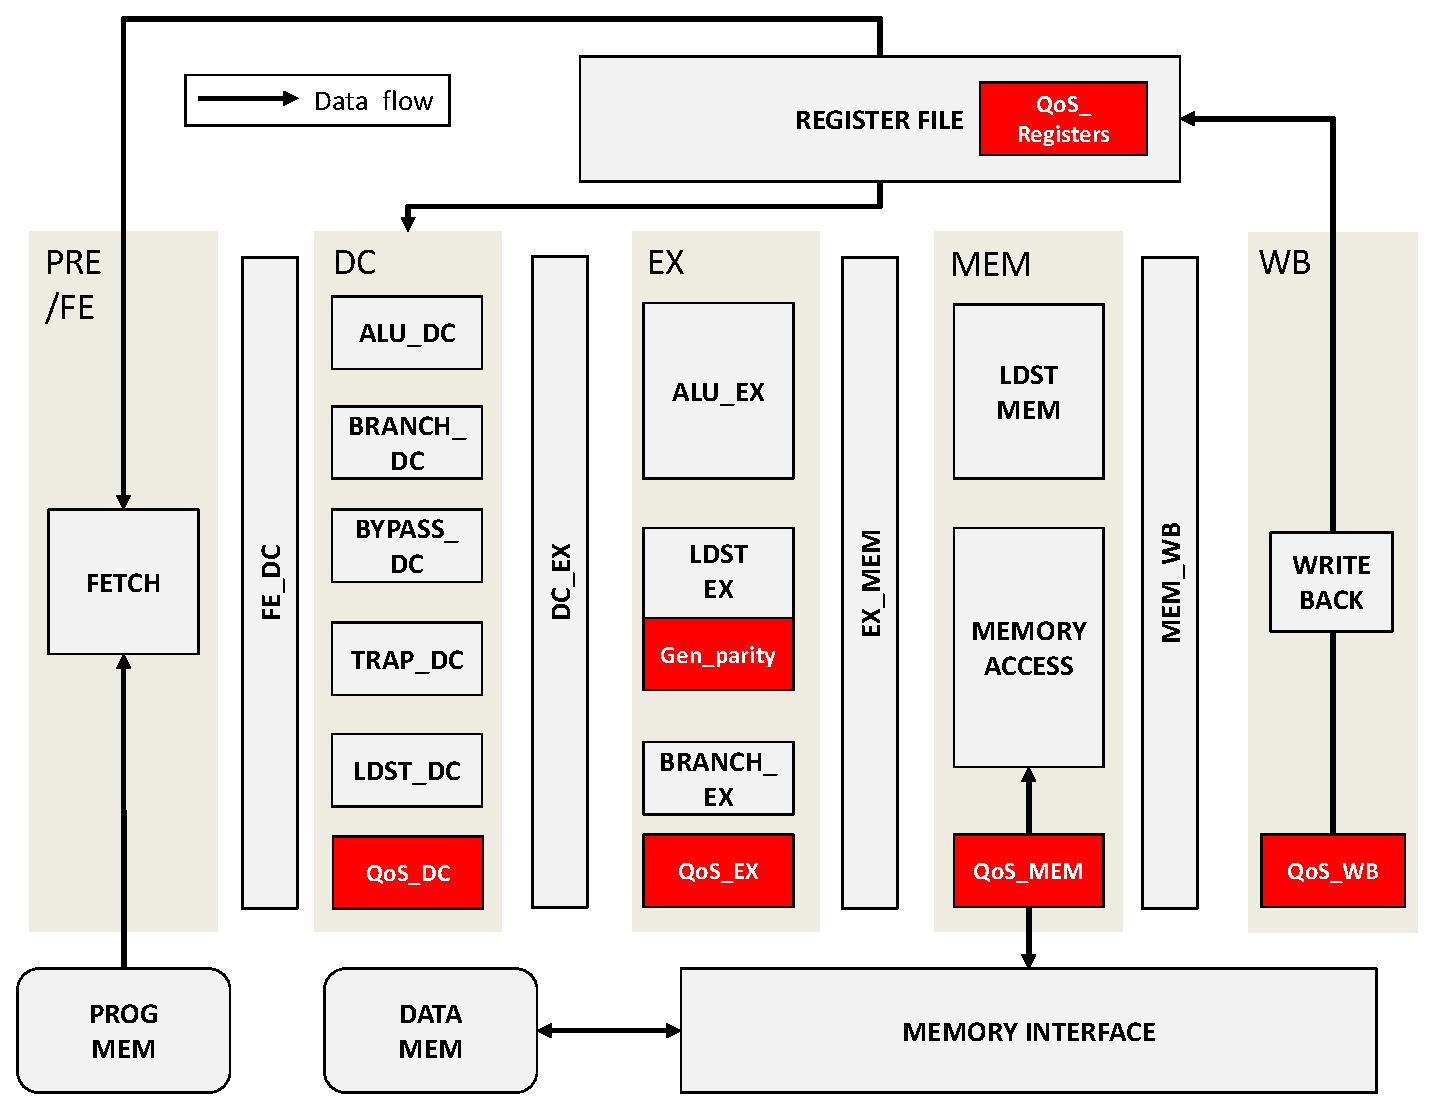
\includegraphics[width=80mm]{./eps/qos_processor}
\caption{Microarchitecture of RISC processor with enhancements for statistical based error confinement}
\vspace{-3mm}
\label{fig:qos_processor}
\end{figure}

\begin{figure}
\centering
\includegraphics[width=90mm]{./eps/qos_arch_explain_date16}
\caption{Introduced modules and their functionality}
\vspace{-3mm}
\label{fig:qos_arch_explain}
\end{figure}
%\vspace{-5mm}

%This has to go in the results
%\begin{figure}
%\centering
%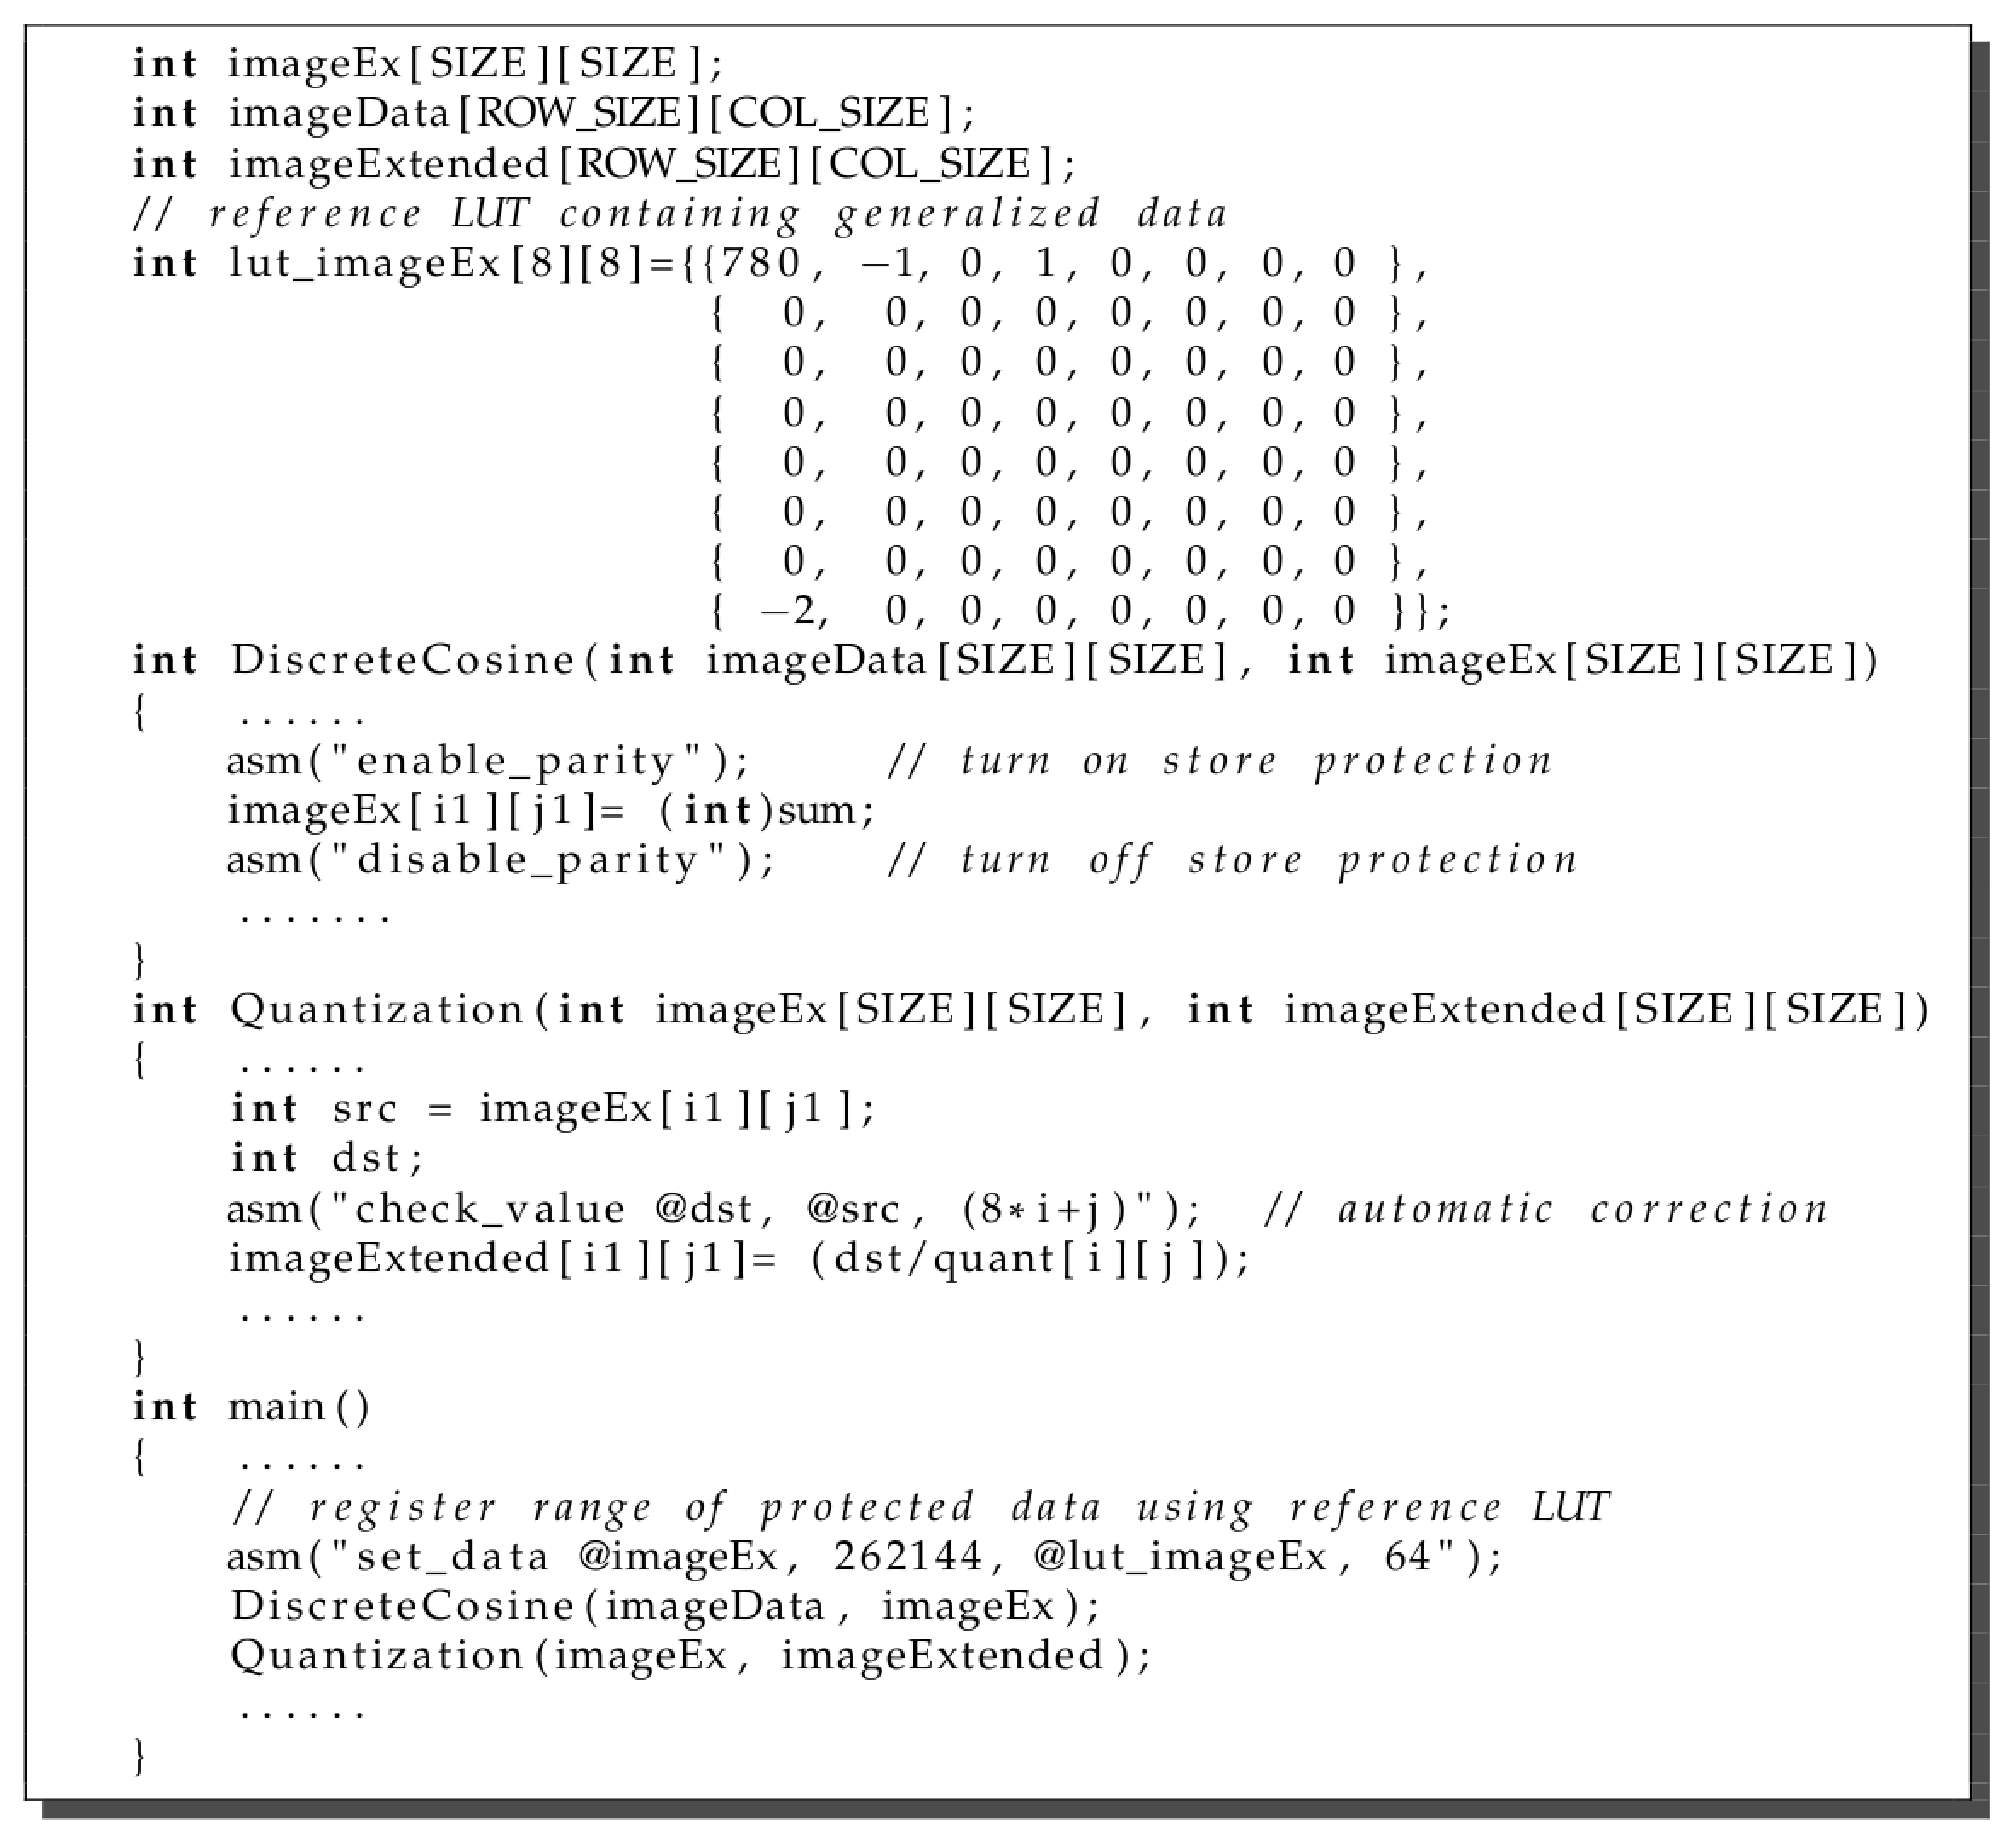
\includegraphics[width=90mm]{./eps/qos_program}
%\caption{Programming example with custom instructions for DCT}
%\label{fig:qos_program}
%\end{figure}

%This has to go in the results
%The architecture is synthesized at 25MHz under 65nm Faraday technology. Table \ref{tab:qos_overhead} presents the synthesis result compared to the original processor. It is observed that the architectural extension incurs huge overheads on the original processor in area and power. Further investigation reviews that the logic and registers which record the memory range of protected data, LUT and parity encoding contribute to such overhead. Additionally, such overhead enables the generic programming environment for similar algorithms, which exhibits the trade-off between hardware usage and programming complexity. However, great saving is resulted from the memory usage as the analysis in Section \ref{sec::soft_overhead}. In terms of critical path, the timing cost only has 4.2\% increment since the longest path of the original design, which goes through the hardware multiplier, remains almost unchanged.

%\begin{table}[hbt]
%\begin{center}
%\caption{Overheads for architecture extension}
%     \label{tab:qos_overhead}
%\begin{tabular}{|c|c|c|c|c|c|}\hline 
%                  & \multicolumn{2}{c|}{\textbf{Area}} & \multicolumn{2}{c|}{\textbf{Power}} & \textbf{Critical} \\ 
%                  & \multicolumn{2}{c|}{\textbf{(NAND equiv.)}} & \multicolumn{2}{c|}{\textbf{($\mu$Watt)}} & \textbf{path} \\ %%\cline{2-5}
%                  & Comb. & Seq. & Dynamic & Leakage & (ns) \\\hline
%Original          & 11789         & 6187       & 206     & 65      & 6.12 \\\hline
%QoS extension     & 26519         & 10663      & 349     & 124     & 6.38 \\\hline
%Increase (\%)     & 124.9         & 72.3       & 69.4    & 90.8    & 4.2  \\\hline
%\end{tabular}
%\end{center}
%\end{table}
